
%-----------------------------------------------%

% PREAMBLE %

%-----------------------------------------------%
\documentclass[a4paper,12pt]{article}

% Packages
\usepackage{textcomp}
\usepackage{gensymb}
\usepackage{graphicx}
\usepackage{amsmath}
\usepackage{geometry}
\usepackage{fancyhdr}
\usepackage{setspace}
\usepackage{titlesec}  % For title formatting
\usepackage{tocloft}
\usepackage{xcolor}
\usepackage{enumitem}
\usepackage{float}


% Header and Footer
\pagestyle{fancy}
\fancyhf{}
\fancyhead[L]{Abereni Opuiyo}
\fancyhead[C]{PHY121}
\fancyhead[R]{\thepage}
\fancyfoot[L]{Final Project: Physics Illustrated in "Hancock"}
\fancyfoot[R]{\nouppercase{\rightmark}}
\geometry{margin=1.2in}
\setstretch{1.5}


\newcommand*{\justifyheading}{\raggedleft}
\renewcommand{\sectionmark}[1]{\markright{#1}}
\renewcommand{\footrulewidth}{0.1pt}% default is 0pt

% Table of Contents
\renewcommand{\contentsname}{Table of Contents}
\renewcommand{\cftsecleader}{\cftdotfill{\cftdotsep}}



% Title Formatting

\titleformat{\section}
	{\normalfont\huge\bfseries\justifyheading}
	{\thesection}
	{1em}{}
	

\titleformat{\subsection}
	{\normalfont\Large\bfseries}
	{\thesubsection}
	{1em}{}
	[{\titlerule[1.8pt]}]

% Cover Page
\title{
    \vspace{5cm} % Adjust vertical space
    
\includegraphics[width=0.55\textwidth]{dutchess-logo-blue.png} \\ % Add your logo here (change "logo.png" to the actual filename)
    \vspace{1cm} % Adjust vertical space after the logo
    \textbf{\Huge Final Project: Physics Illustrated in "Hancock"} \\
    \vspace{1cm} % Adjust vertical space
    \large PHY121 \\
    \vspace{0.5cm} % Adjust vertical space
    \large	October, 4th, 2024 \\ 
		\vspace{.5cm}
		\large Professor Renee Lathrop 
}
\author{Abereni Opuiyo}
\date{}
%-----------------------------------------------%

% TITLE PAGE %

%-----------------------------------------------%
\begin{document}
\maketitle
	\thispagestyle{plain}
\newpage

%-----------------------------------------------%

% Table of Contents  %

%-----------------------------------------------%
% Start page numbering from the Table of Contents

\setcounter{secnumdepth}{0}
\setcounter{page}{1}  % Start counting from 1
\tableofcontents
\thispagestyle{fancy}
\newpage

%-----------------------------------------------%
\section{Unit 1}

\vspace{-0.5cm}
\singlespacing

\subsection{Scene Analysis}

\textbf{Duration}: 4:50 - 12:00

\vspace{0.3cm}
\noindent\textbf{Summary:} \par
Shortly after being woken up from a drunken slumber, Hancock flies into the air and pursues a getaway vehicle a few miles away. After terrorizing the crooks by swinging their car in the air like a toy, Hancock tosses the car into the air and onto a building.
\par


\vspace{0.3cm}
\noindent\textbf{Concepts Demonstrated} \par
This scene demonstrates many concepts in physics, specifically, \emph{kinematics in one
	dimension} as Hancock flies in the air. The distance Hancock travels could
	also cover \emph{unit conversions}, since we would need to convert the miles
	he travels into meters to use in the equations for kinematics. \emph{Free falling bodies} is also covered as Hancock throws the car into the air.


\vspace{0.3cm}
\noindent\textbf{Is this "Good Physics"?} \par

The movie never explains how Hancock is able to overcome the force of gravity
	and maintain flight in the air. In real life, he’d fall straight to the ground
	shortly after attempting to take off.

\subsection{Problem 1}
Hancock takes off and flies directly after the getaway vehicle, covering a distance of 8 miles. His initial speed is 30 m/s, and he decelerates at a constant rate of -15 m/s$^2$ when approaching the vehicle. Assume no air resistance and ignore the forces that would be required for flight. 


\noindent\textbf{A) Convert 8 miles to meters.} \\

\noindent\textbf{Solution:}

\begin{figure}[H]
    \centering
    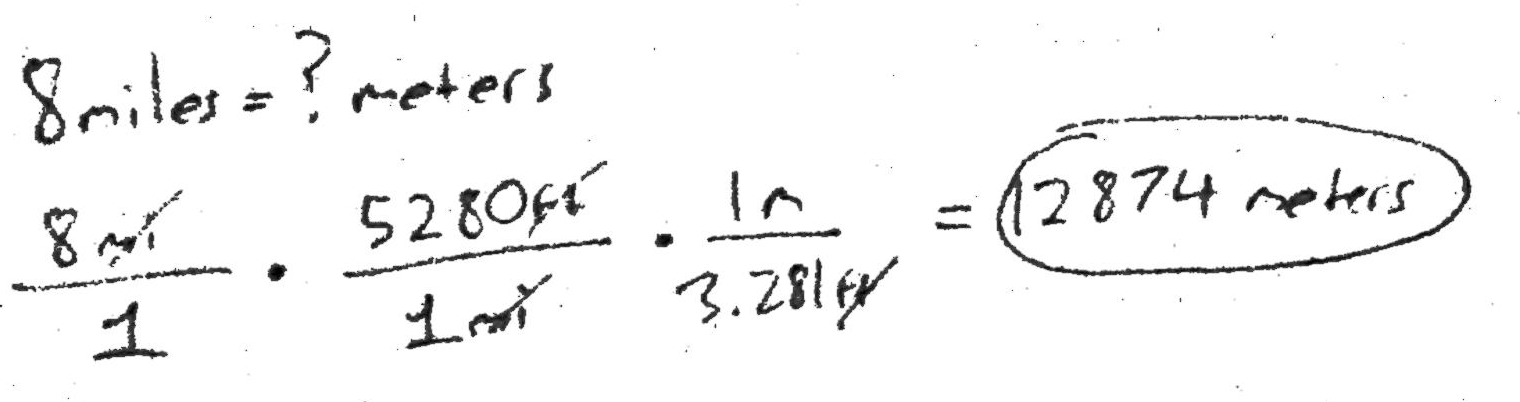
\includegraphics[width=0.8\textwidth]{U1_P1_A} % Example of adding a figure
\end{figure} \\


\noindent\textbf{B) How long does it take Hancock to travel 8 miles if he maintains a speed of 30 m/s?} \\

\noindent\textbf{Solution:}

\begin{figure}[H]
    \centering
    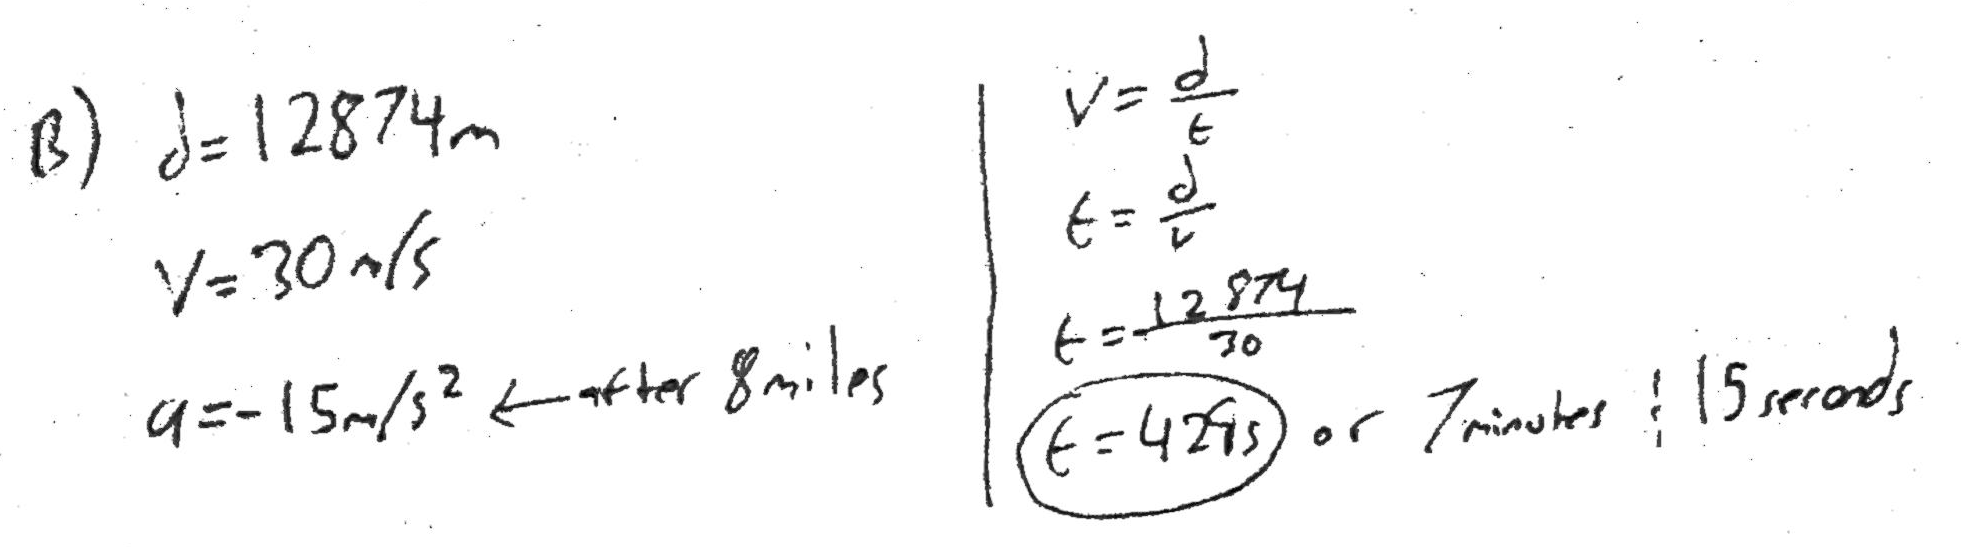
\includegraphics[width=0.8\textwidth]{U1_P1_B} % Example of adding a figure
\end{figure}


\noindent\textbf{C) Once he reaches the vehicle, how long does it take for Hancock to come to a complete stop with a deceleration of -15 m/s$^2$?} \\

\noindent\textbf{Solution:}

\begin{figure}[H]
    \centering
    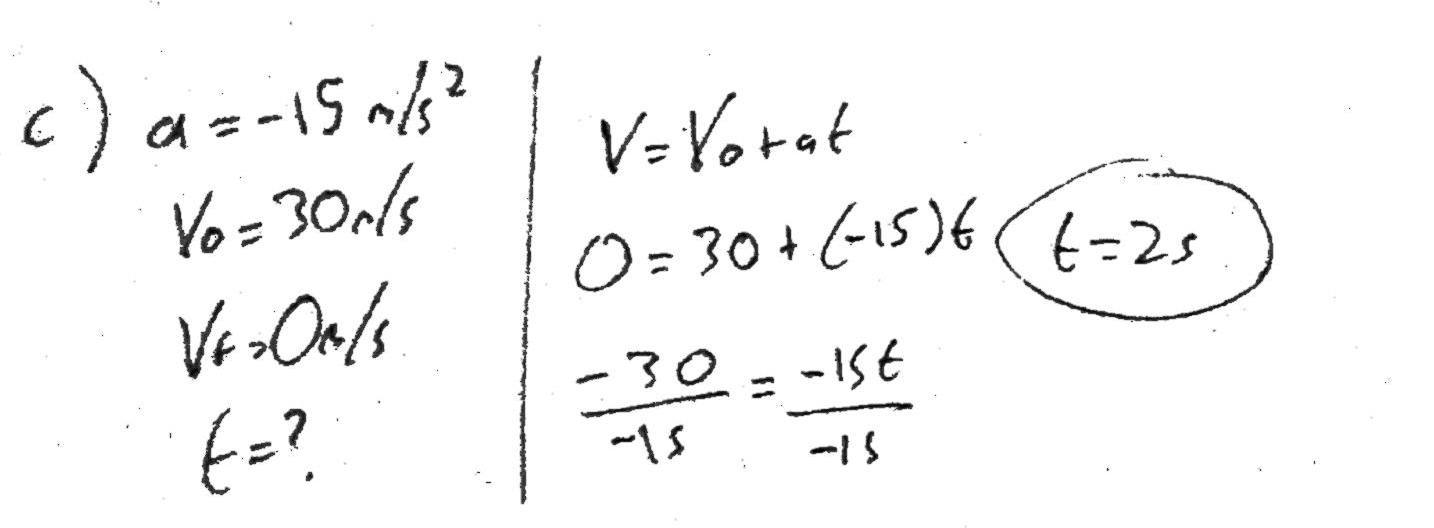
\includegraphics[width=0.8\textwidth]{U1_P1_C} % Example of adding a figure
\end{figure}


\noindent\textbf{D) How far does Hancock travel while decelerating to a stop?} \\

\noindent\textbf{Solution:}

\begin{figure}[H]
    \centering
    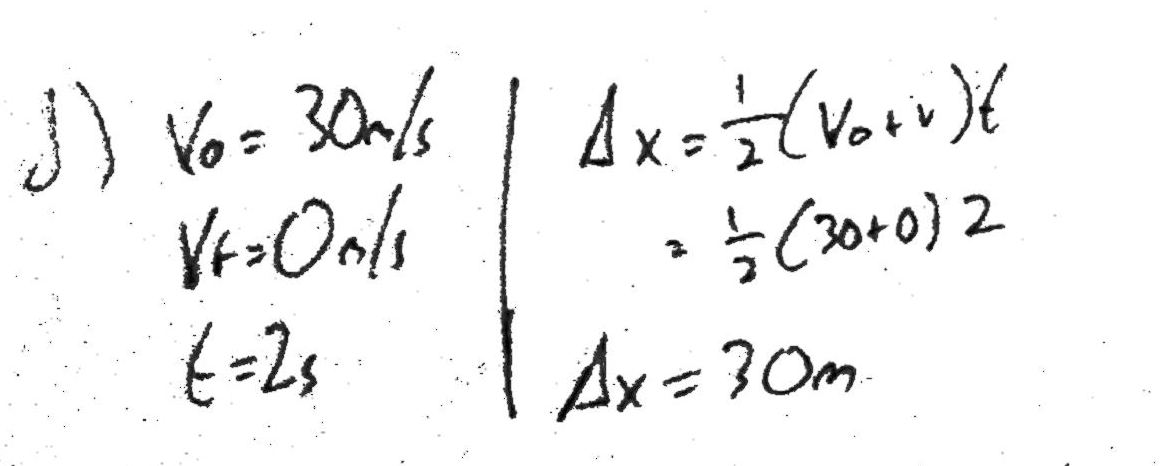
\includegraphics[width=0.8\textwidth]{U1_P1_D} % Example of adding a figure
\end{figure}

\newpage

\noindent\textbf{E) Calculate the total distance Hancock covers from takeoff until he stops.} \\

\noindent\textbf{Solution:}

\begin{figure}[H]
    \centering
    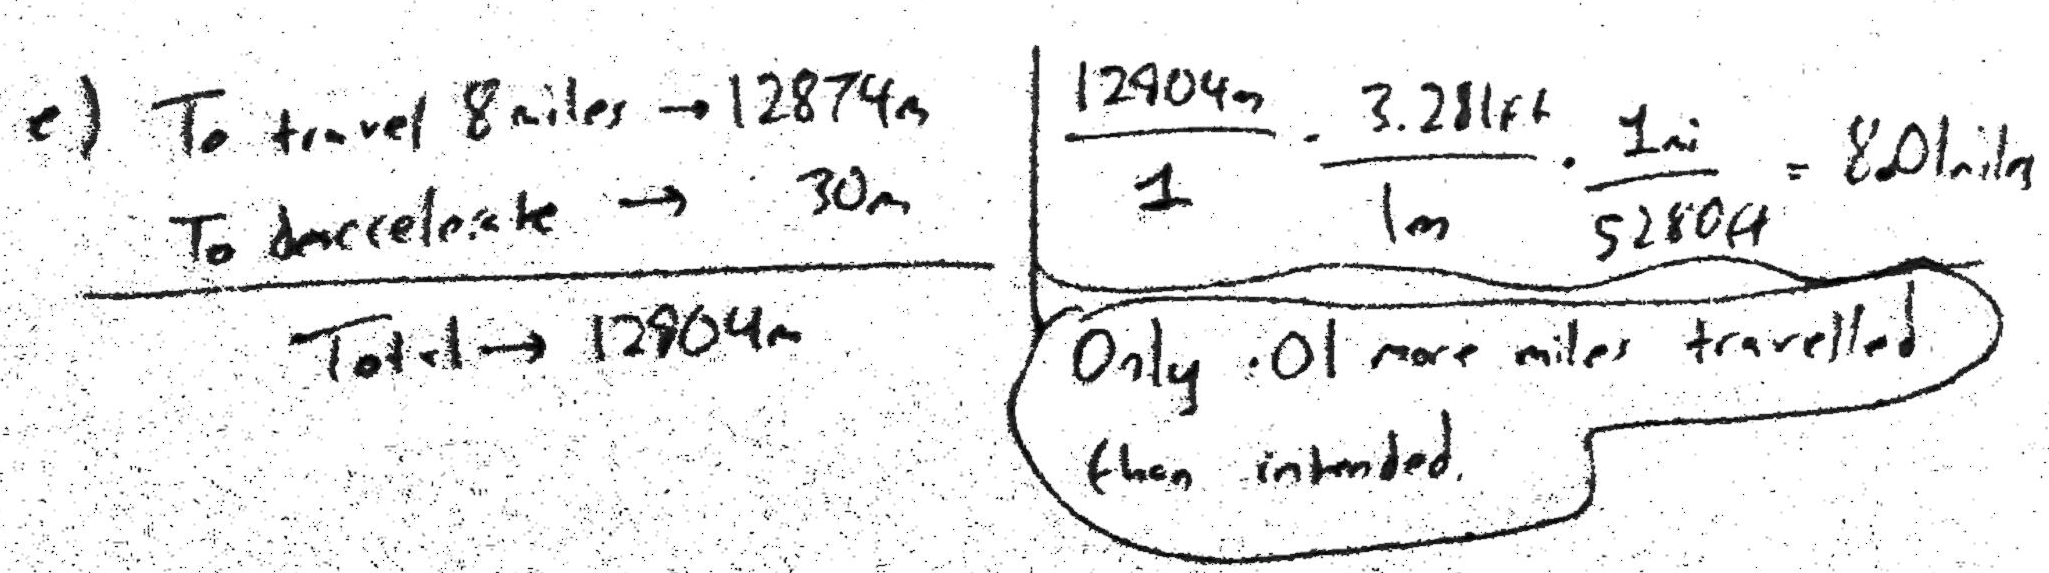
\includegraphics[width=0.8\textwidth]{U1_P1_E} % Example of adding a figure
\end{figure}

%-----------------PROBLEM 2--------------------------%

\subsection{Problem 2}

Assume Hancock throws the car straight up into the air from the ground to scare the crooks at an initial velocity of 20 m/s. He catches them a short time later. \\

\noindent\textbf{A) Calculate the car's acceleration immediately after Hancock releases it.} \\

\noindent\textbf{Solution:}

\begin{figure}[H]
    \centering
    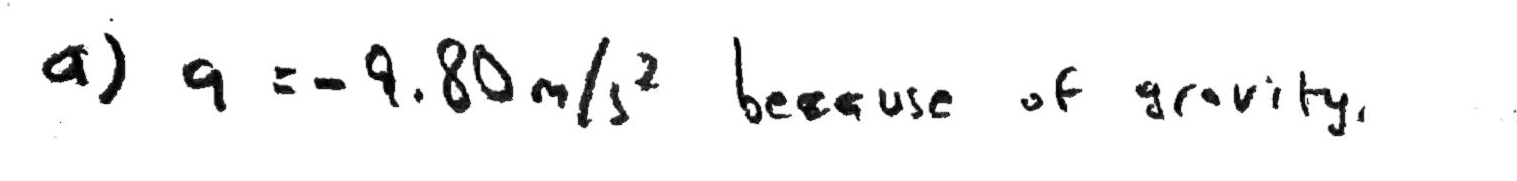
\includegraphics[width=0.8\textwidth]{U1_P2_A} % Example of adding a figure
\end{figure}


\noindent\textbf{B) Calculate the displacement of the car.} \\

\noindent\textbf{Solution:}

\begin{figure}[H]
    \centering
    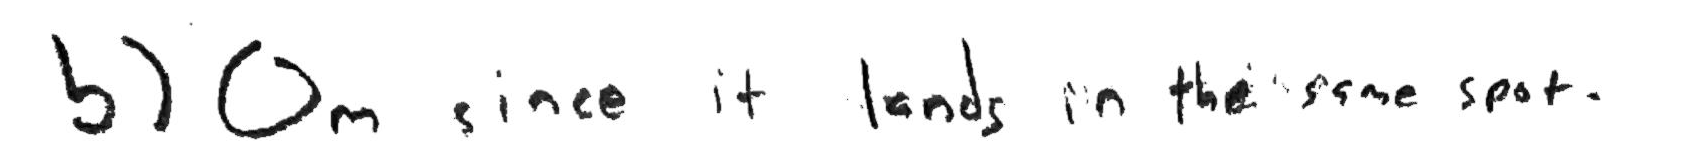
\includegraphics[width=0.8\textwidth]{U1_P2_B} % Example of adding a figure
\end{figure}


\noindent\textbf{C) Calculate the maximum height the car reaches above the ground.}\\ 

\noindent\textbf{Solution:}

\begin{figure}[H]
    \centering
    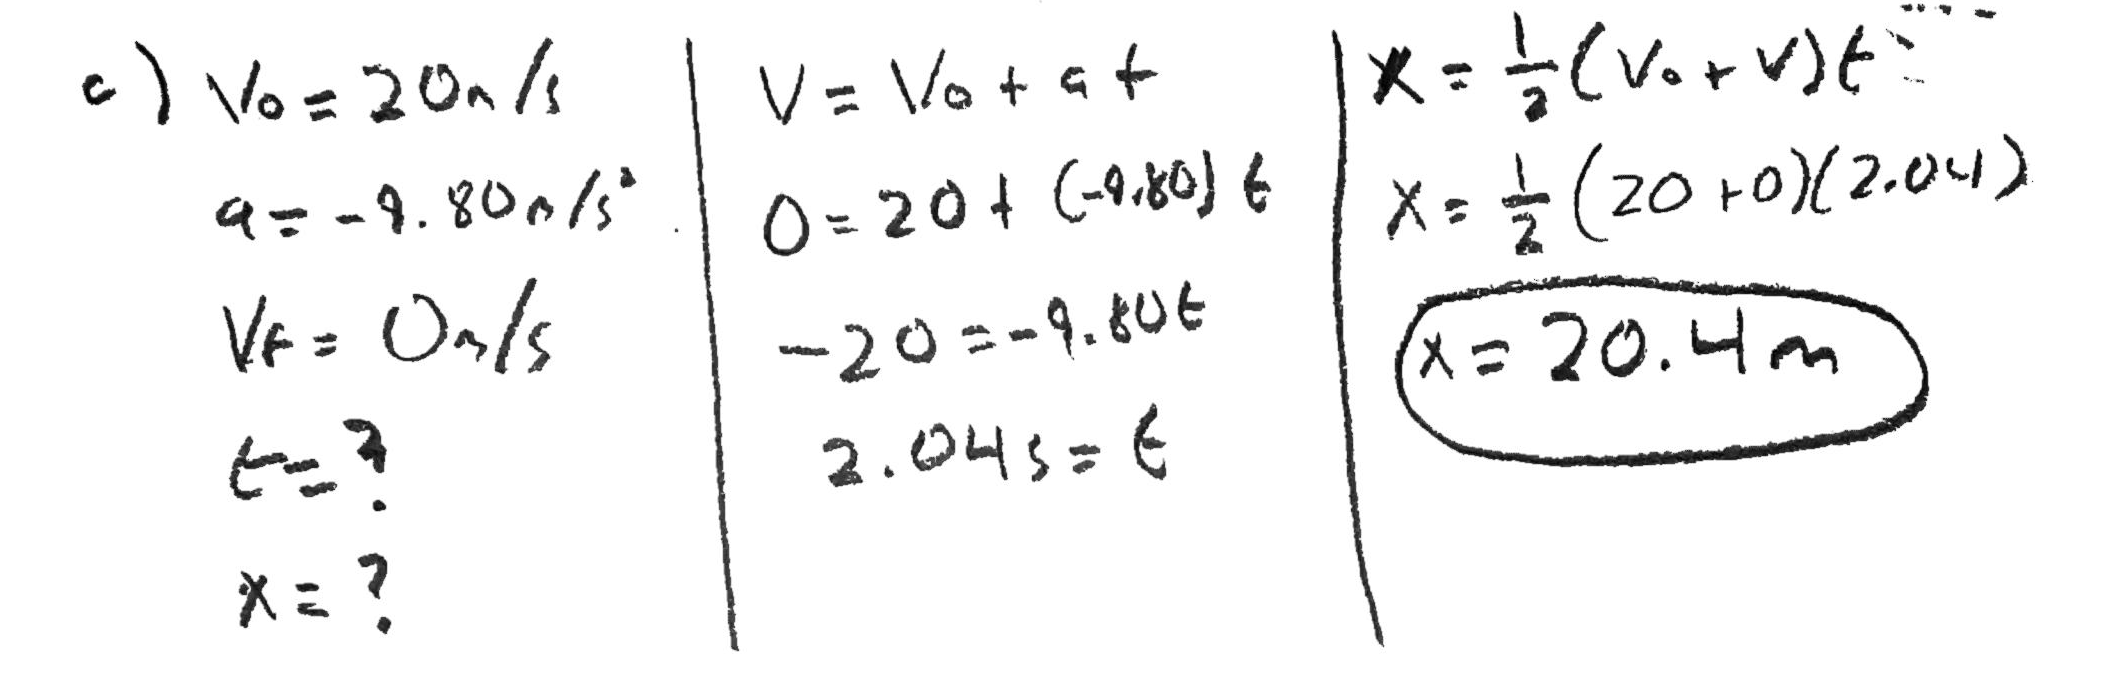
\includegraphics[width=0.8\textwidth]{U1_P2_C} % Example of adding a figure
\end{figure}

%\vspace{-0.5cm}

\noindent\textbf{D) How long does it take the car to reach its maximum height? What's the total time in the air?} \\

\vspace{-0.2cm}

\noindent\textbf{Solution:}

\begin{figure}[H]
    \centering
    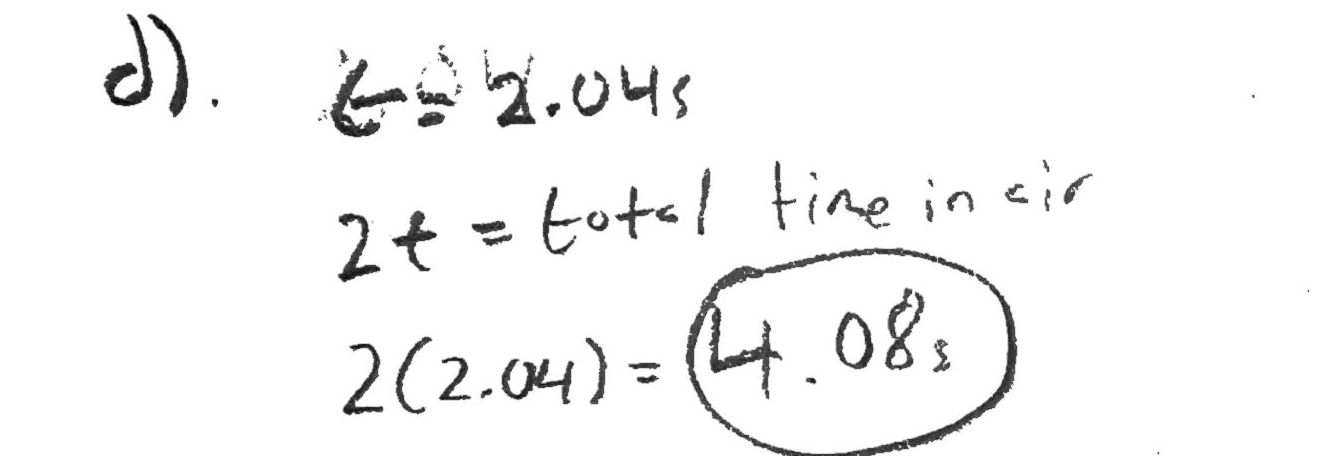
\includegraphics[width=0.8\textwidth]{U1_P2_D} % Example of adding a figure
\end{figure}

\newpage

%==============UNIT 2==================%

\section{Unit 2}

\vspace{-0.5cm}
\singlespacing

\subsection{Scene Analysis}

\textbf{Duration}: 26:00 - 28:00

\vspace{0.3cm}
\noindent\textbf{Summary:} \par
After being taunted by a 10 year old, Hancock loses his patience and throws the kid into the air. While in the air, Hancock finishes a conversation and walks a short distance, positioning himself to catch the child just before he hits the ground.
\par


\vspace{0.3cm}
\noindent\textbf{Concepts Demonstrated} \par
This scene is an excellent example of kinematics in two dimensions. Hancock accounts for the horizontal distance that the kid travels in the air to catch him at just the right moment.  

\vspace{0.3cm}
\noindent\textbf{Is this "Good Physics"?} \par

The movie never explains how Hancock is able to overcome the force of gravity
	and maintain flight in the air. In real life, he’d fall straight to the ground
	shortly after attempting to take off.

\subsection{Problem 1}
Assume Hancock throws the child vertically upward with an initial velocity of 58 m/s at an angle of 87$^\circ$. Neglect air resistance. \\


\noindent\textbf{A) Calculate the initial vertical and horizontal components of the child's velocity.} \\

\noindent\textbf{Solution:}

\begin{figure}[H]
    \centering
    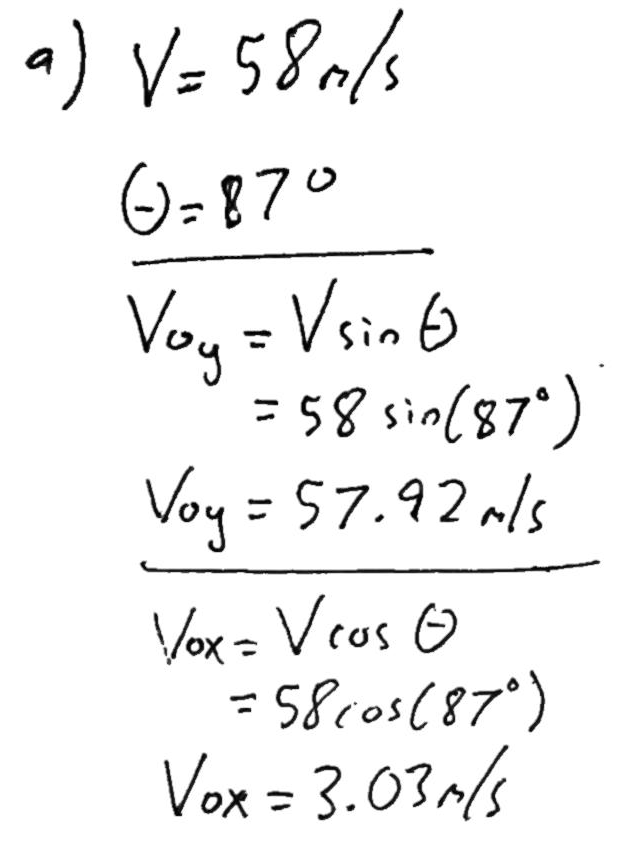
\includegraphics[width=0.3\textwidth]{U2_P1_A} % Example of adding a figure
\end{figure}

\newpage

\noindent\textbf{B) Calculate the maximum height the child reaches. \emph{Could he see his house from up there?}} \\

\noindent\textbf{Solution:}

\begin{figure}[H]
    \centering
    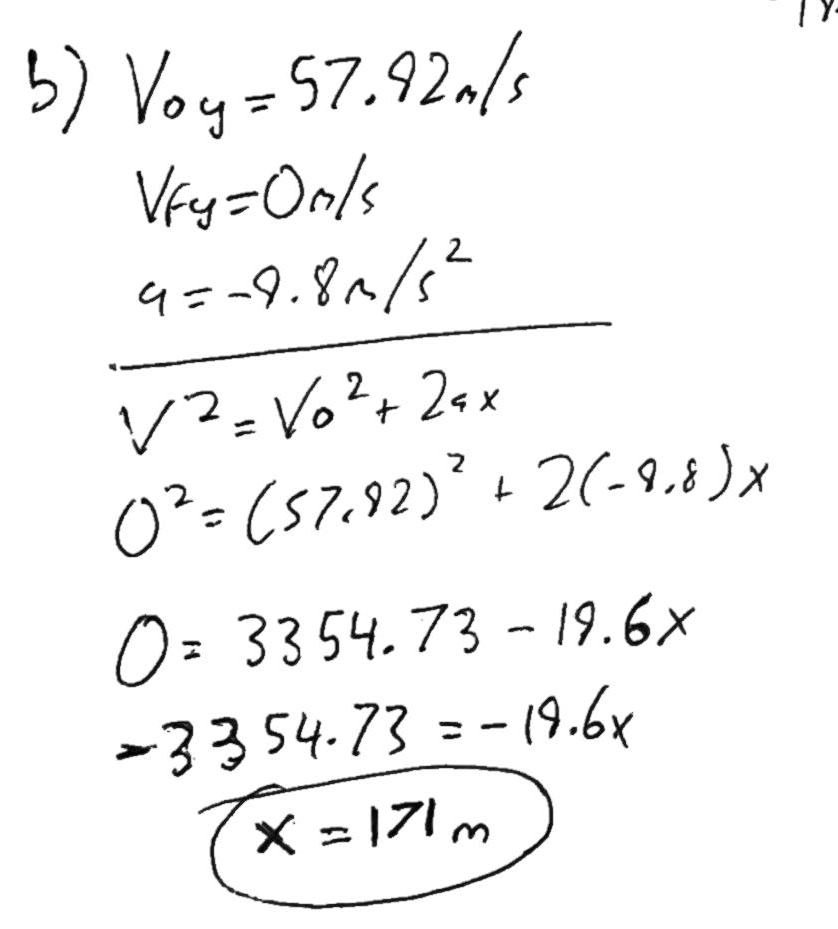
\includegraphics[width=0.3\textwidth]{U2_P1_B} % Example of adding a figure
\end{figure}

\noindent\textbf{C) How long does it take the child to reach maximum height? And to come back down? \emph{Is that enough time to think about the mistake he made?}} \\

\noindent\textbf{Solution:}

\begin{figure}[H]
    \centering
    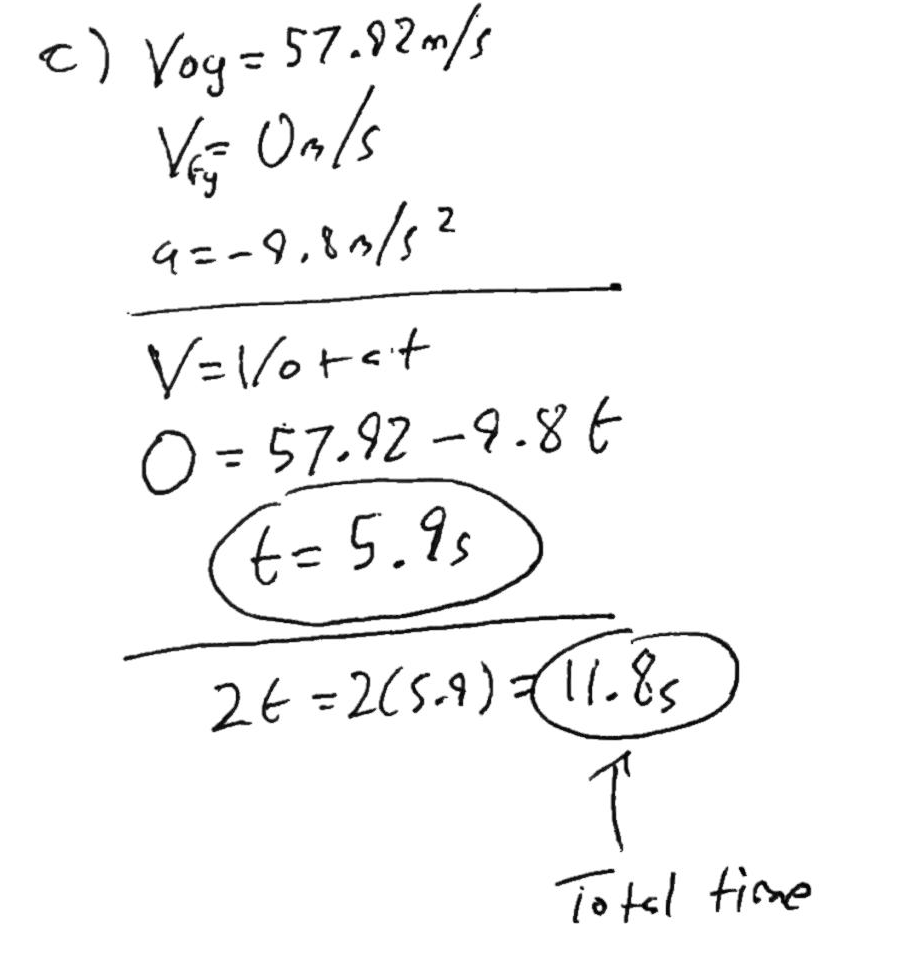
\includegraphics[width=0.3\textwidth]{U2_P1_C} % Example of adding a figure
\end{figure}

\noindent\textbf{D) How far does Hancock have to walk to catch the kid?} \\

\noindent\textbf{Solution:}

\begin{figure}[H]
    \centering
    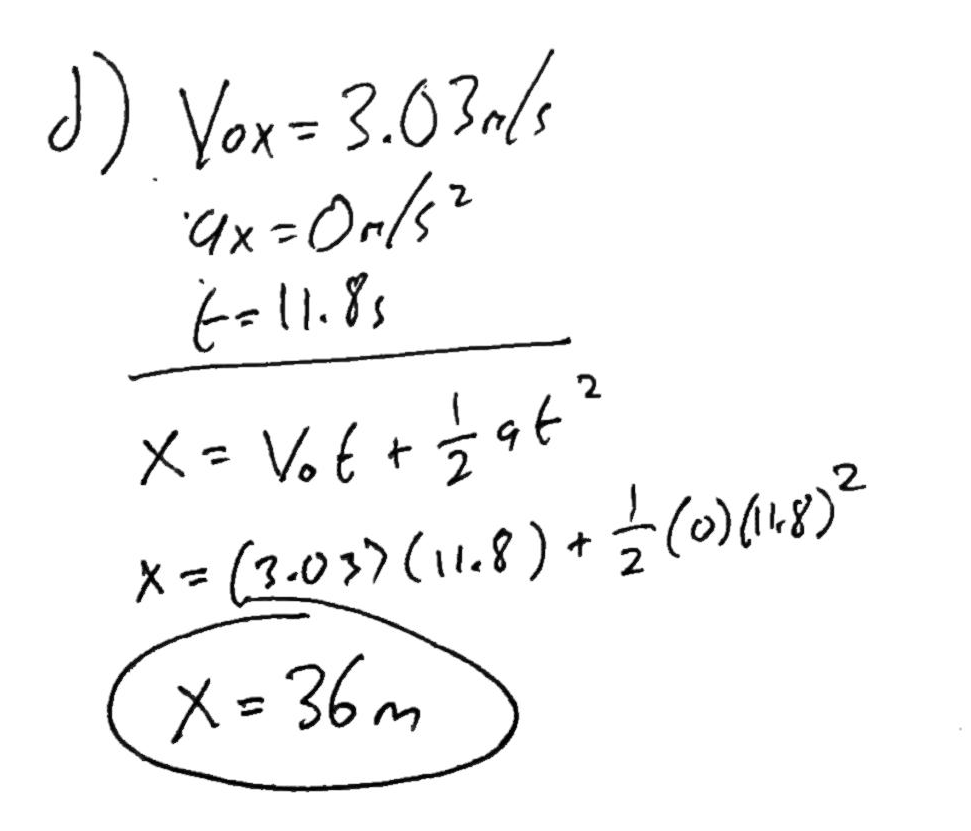
\includegraphics[width=0.3\textwidth]{U2_P1_D} % Example of adding a figure
\end{figure}

%=====================UNIT 3===================%
\section{Unit 3}

\vspace{-0.5cm}
\singlespacing

\subsection{Scene Analysis}

\textbf{Duration}: 17:54 - 24:00

\vspace{0.3cm}
\noindent\textbf{Summary:} \par
After preventing a train from hitting the car of public relations manager, Ray, Hancock carries the car back to Ray's house. When he arrives, he drags the car up a slight incline into the garage. \\
\par


\vspace{0.3cm}
\noindent\textbf{Concepts Demonstrated} \par
This scene demonstrates work done by a force, kinetic energy and gravitational potential energy as Hancock drags the car up to Ray's garage.  

\subsection{Problem 1}
Assume Hancock drags Ray's 1500 kg car up a 5$^\circ$ incline over a distance of 50 m to the garage. The frictional force opposing the motion is 3000 N, and Hancock maintains a constant speed of 4 m/s as he moves the car up the incline. \\


\noindent\textbf{A) Calculate the work done by Hancock to overcome the frictional force as he drags the car up the incline.} \\

\noindent\textbf{Solution:}

\begin{figure}[H]
    \centering
    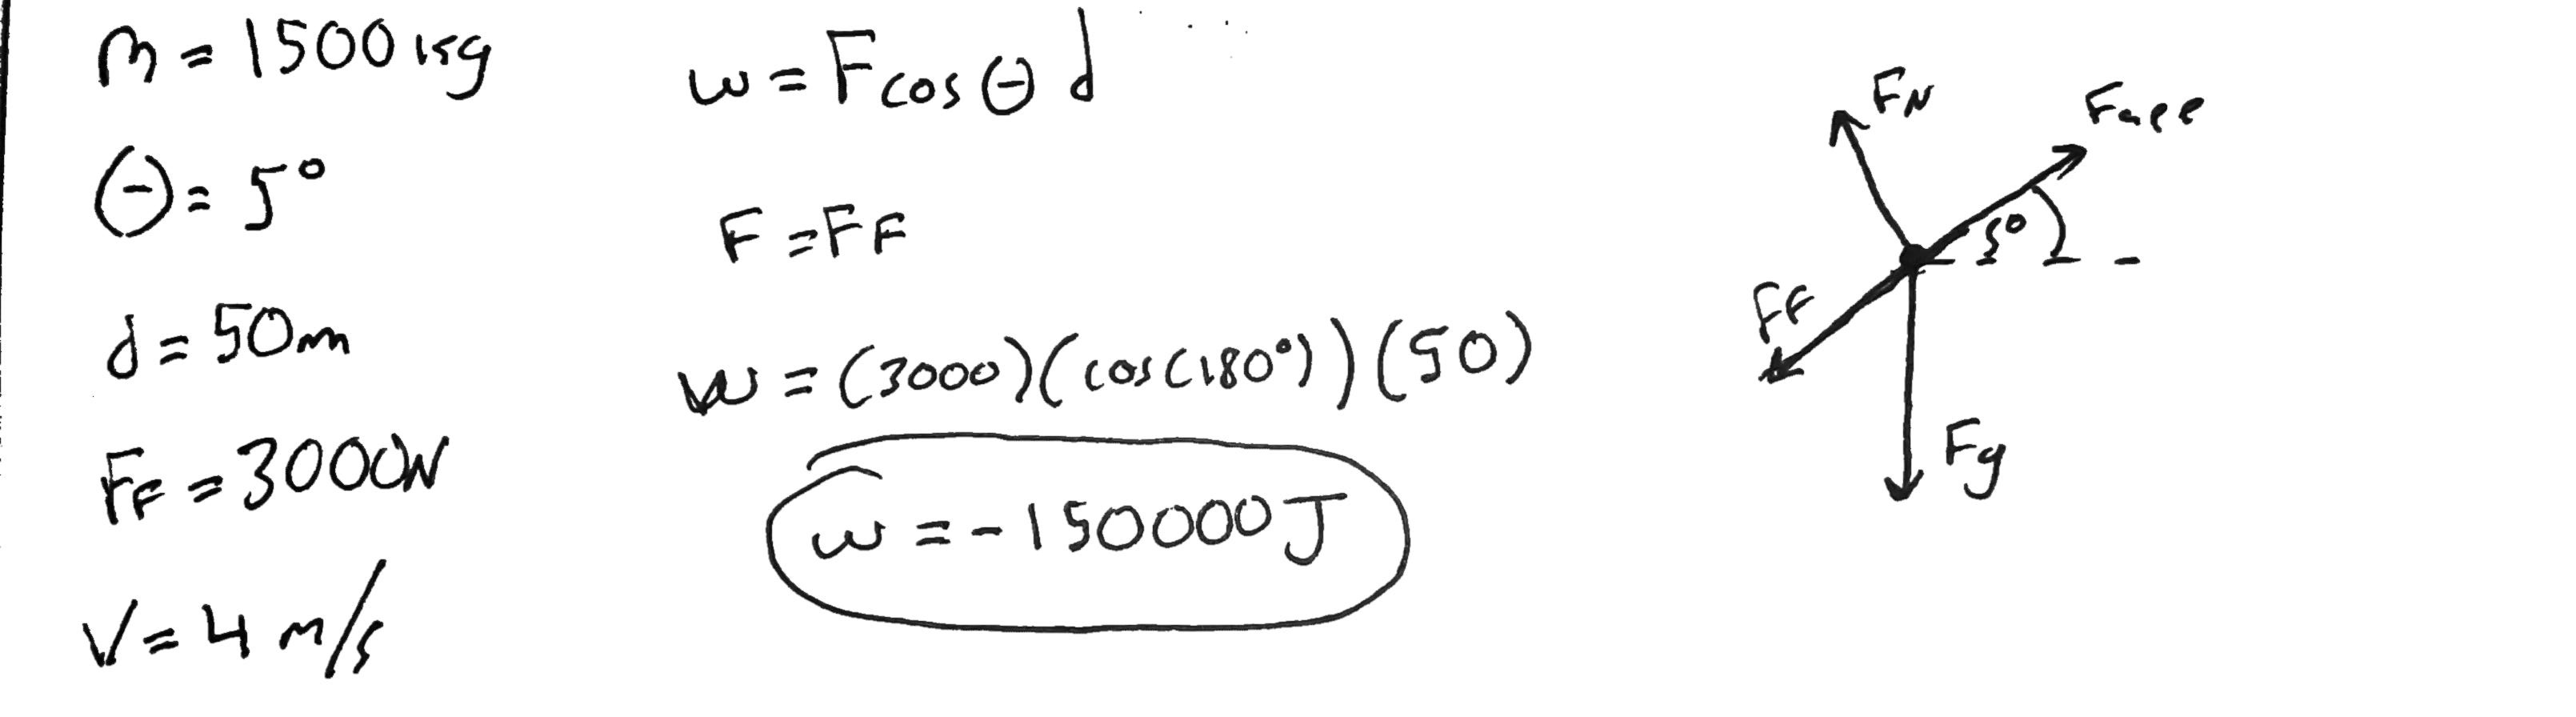
\includegraphics[width=0.5\textwidth]{U3_P1_A} % Example of adding a figure
\end{figure} 

\newpage

\noindent\textbf{B) Calculate the change in gravitational potential energy of the car as it is raised to the height of the incline.} \\

\noindent\textbf{Solution:}

\begin{figure}[H]
    \centering
    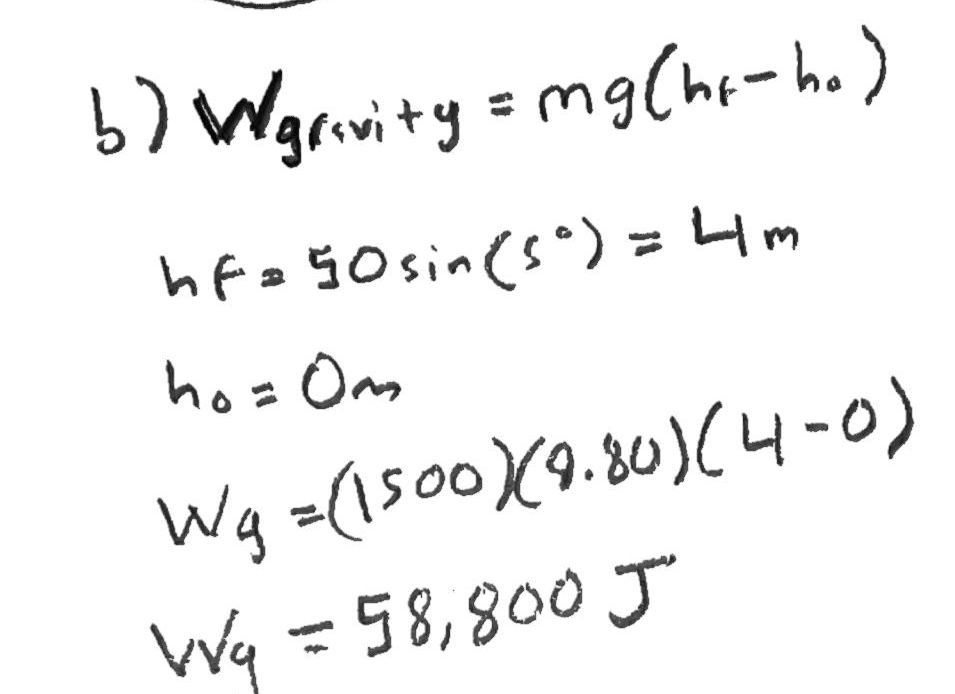
\includegraphics[width=0.5\textwidth]{U3_P1_B} % Example of adding a figure
\end{figure}

\noindent\textbf{C) Calculate the total work Hancock performs to move the car up the incline.} \\

\noindent\textbf{Solution:}

\begin{figure}[H]
    \centering
    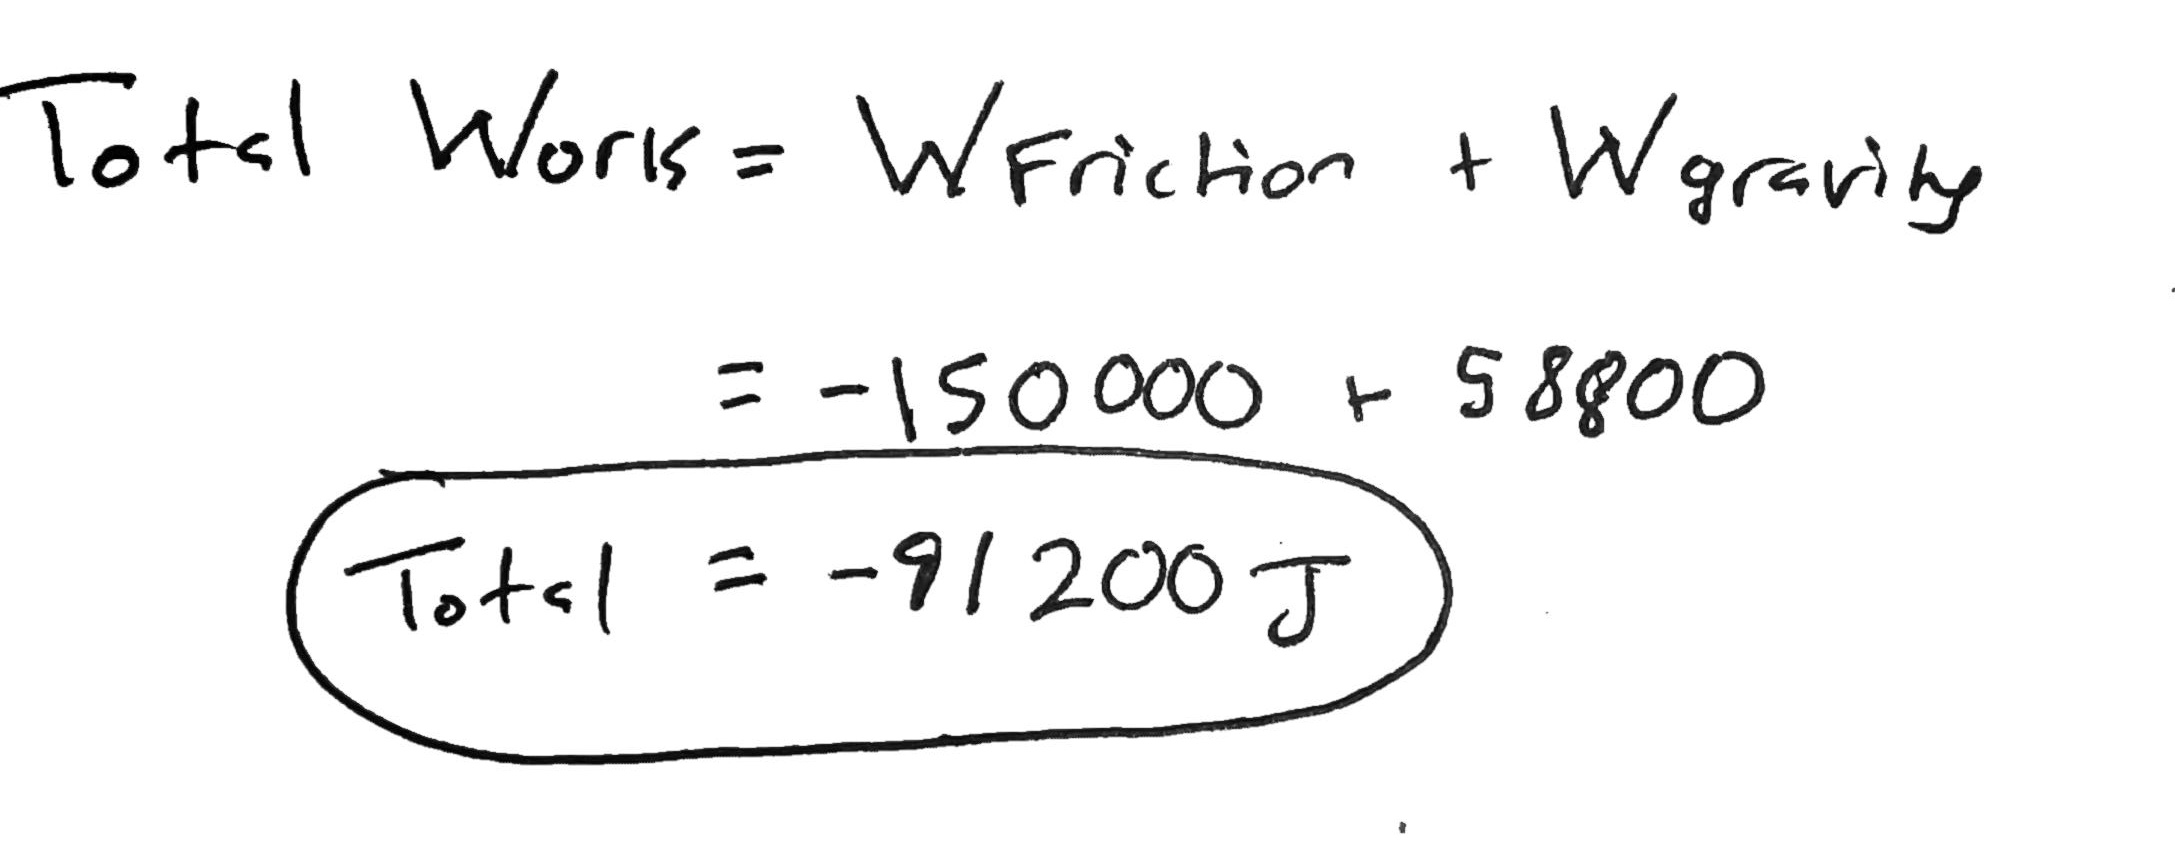
\includegraphics[width=0.5\textwidth]{U3_P1_C} % Example of adding a figure
\end{figure}

\noindent\textbf{D) Calculate the change in kinetic energy of the car as it moves up the incline.} \\

\noindent\textbf{Solution:}

\begin{figure}[H]
    \centering
    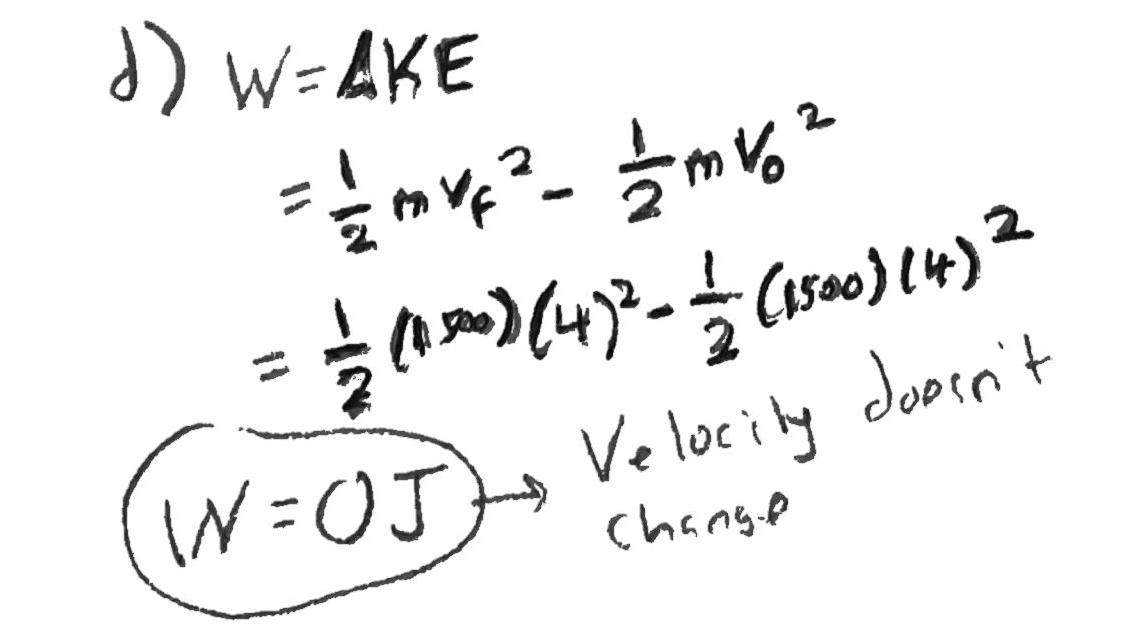
\includegraphics[width=0.5\textwidth]{U3_P1_D} % Example of adding a figure
\end{figure}

\newpage

\noindent\textbf{E) What is the total energy lost to friction as Hancock drags the car up the incline?} \\

\noindent\textbf{Solution:}

\begin{figure}[H]
    \centering
    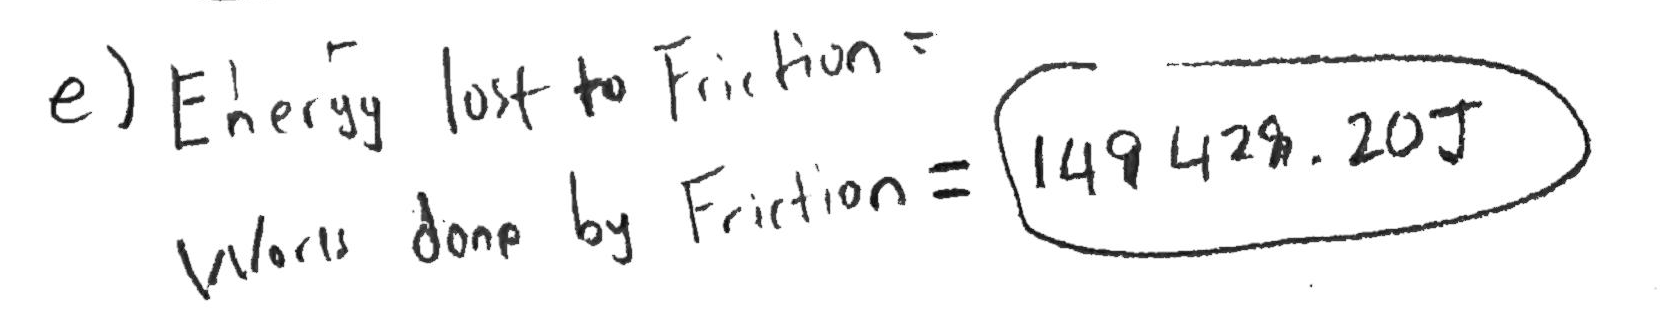
\includegraphics[width=0.5\textwidth]{U3_P1_E} % Example of adding a figure
\end{figure}


\noindent\textbf{F) Draw an FBD diagram of the problem} \\

\noindent\textbf{Solution:}

\begin{figure}[H]
    \centering
    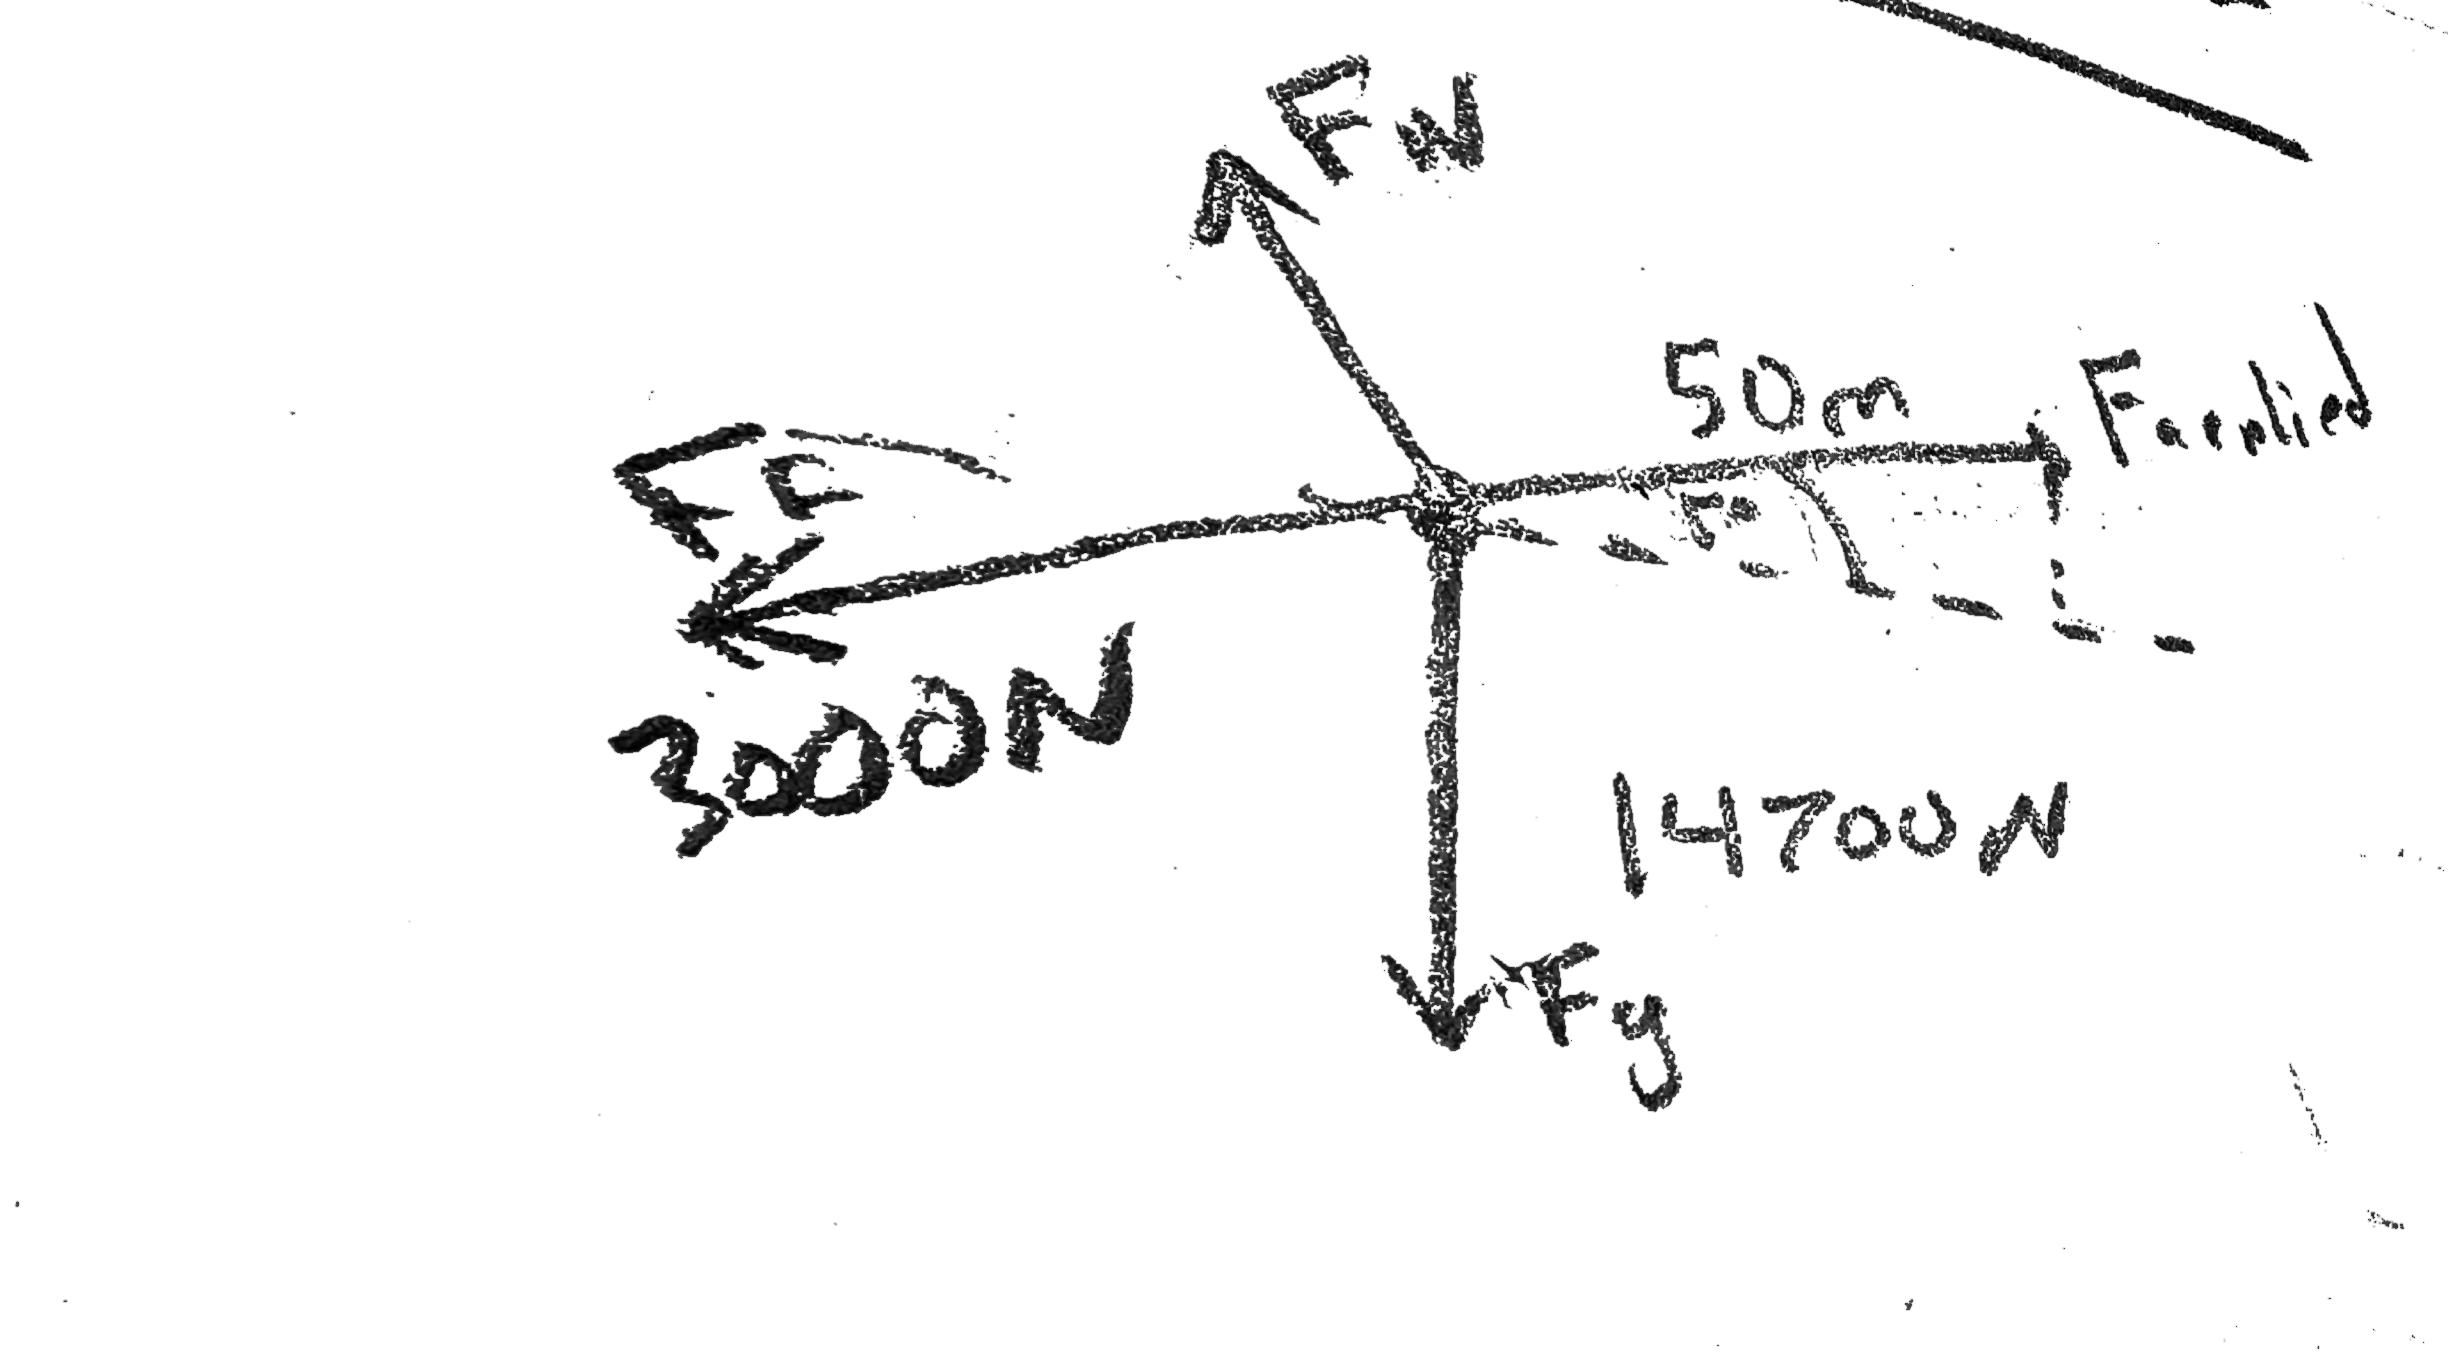
\includegraphics[width=0.5\textwidth]{U3_P1_F} % Example of adding a figure
\end{figure}
\end{document}
